\documentclass{beamer}                             % presentation
% \documentclass[draft]{beamer}                    % improves compile time
% \documentclass[11pt, handout]{beamer}            % handout
\usepackage[utf8]{inputenc}                        % utf8
\usepackage[T1]{fontenc}                           % fix font encoding
\usepackage[english]{babel}                        % language
\usepackage{bm, mathtools}                         % extra math packages
\usepackage{graphicx, subcaption}                  % images
\usepackage{tikz, pgfplots}                        % plots and graphs
\usepackage[style=ieee]{biblatex}                  % bibliography
\usepackage{geometry, hyperref, enumitem}          % misc.
\usepackage[cache=true]{minted}                    % source code
\usepackage[autostyle, english=american]{csquotes} % quotes

\usetikzlibrary{positioning}                       % advanced positioning
\pgfplotsset{compat=newest}                        % version of pgfplots

\graphicspath{{./figures/}}
\addbibresource{references.bib}

\setminted[]{
  linenos=true,
  breaklines=true,
  encoding=utf8,
  fontsize=\normalsize,
  frame=lines,
  framesep=2mm
}

% https://tex.stackexchange.com/questions/343494/minted-red-box-around-greek-characters
\makeatletter
\AtBeginEnvironment{minted}{\dontdofcolorbox}
\def\dontdofcolorbox{\renewcommand\fcolorbox[4][]{##4}}
\makeatother

% serif font in math mode
\usefonttheme[onlymath]{serif}
% customize \item in itemize
\setitemize{label={},itemsep=0.5cm}
\setenumerate{label=\arabic*.}

\newcommand{\D}[1]{\, \mathrm{d} #1}
\renewcommand{\vec}[1]{\bm{#1}}
\DeclareMathOperator{\diag}{diag}
\let\trace\relax
\DeclareMathOperator{\trace}{trace}
\DeclareMathOperator{\logdet}{logdet}
\DeclareMathOperator{\chol}{chol}

\DeclareMathOperator*{\argmin}{argmin}

\DeclareMathOperator{\E}{E}
\DeclareMathOperator{\Var}{Var}
\DeclareMathOperator{\Cov}{Cov}
\DeclareMathOperator{\I}{I}
\DeclareMathOperator{\entropy}{H}

%%% colors

\definecolor{lightblue}{HTML}{a1b4c7}
\definecolor{orange}{HTML}{ea8810}
\definecolor{silver}{HTML}{b0aba8}
\definecolor{rust}{HTML}{b8420f}
\definecolor{seagreen}{HTML}{23553c}

\colorlet{lightsilver}{silver!20!white}
\colorlet{darkorange}{orange!85!black}
\colorlet{darksilver}{silver!85!black}
\colorlet{darklightblue}{lightblue!75!black}
\colorlet{darkrust}{rust!85!black}
\colorlet{darkseagreen}{seagreen!85!black}

\hypersetup{
  colorlinks=true,
  linkcolor=darkrust,
  citecolor=darkseagreen,
  urlcolor=darksilver
}

%%% beamer settings

\usetheme{Pittsburgh}
\usecolortheme{dolphin}

% change colors
% https://ramblingacademic.com/2015/12/08/how-to-quickly-overhaul-beamer-colors/
\setbeamercolor{structure}{fg=lightblue}
\setbeamercolor{section in toc}{fg=lightblue}
% change title color
\setbeamercolor{title}{fg=darklightblue}
\setbeamercolor{frametitle}{fg=darklightblue}
\setbeamercolor{framesubtitle}{fg=lightblue}
% change bibliography entry colors
\setbeamercolor{bibliography entry author}{fg=darklightblue}
\setbeamercolor{bibliography entry note}{fg=lightblue}

% hide navigation buttons
\setbeamertemplate{navigation symbols}{}
% table of contents
\setbeamertemplate{sections/subsections in toc}[sections numbered]

% title page
\title[]{Sparse Cholesky Factorization by \\ Greedy Conditional Selection}
\subtitle{}
\author[Huan]
{Stephen Huan}
\institute[Georgia Institute of Technology]
{
  Theory Club
}
\date[]{February 28, 2022}
\subject{Computer Science}

\AtBeginSection[]
{
    \begin{frame}
        \frametitle{Table of Contents}
        \tableofcontents[currentsection]
        \uncover<handout:0>{
          \begin{tikzpicture}[overlay,remember picture]
          \node[above left=2.5cm and 0.1cm] at (current page.south east) {
              
\includegraphics[width=4cm]{
                genshin/chibi/eula/vantage_point.png
              }
          };
          \end{tikzpicture}
        }
    \end{frame}
}

\begin{document}
\frame{
  \titlepage
  \uncover<handout:0>{
    \begin{tikzpicture}[overlay,remember picture]
    \node[above left=0.1cm and 0cm] at (current page.south east) {
        
\includegraphics[width=4cm]{genshin/chibi/ayaka/03_greetings.png}
    };
    \end{tikzpicture}
  }
}

\section{High-level Summary}

\begin{frame}
\frametitle{The Problem: Gaussian Process Regression}
\framesubtitle{}
  \begin{columns}
    \begin{column}{0.6\textwidth}
      \begin{itemize}
        \item<+-> Measurements \( \vec{y}_\text{Tr} \) at
          \( N \) points \( X_\text{Tr} \)

        \item<+-> Estimate unseen data \(
          \vec{y}_\text{Pr} \) at \( X_\text{Pr} \)

        \item<+-> Model as Gaussian process

          \( \rightarrow \) condition on \( \vec{y}_\text{Tr} \)

        \item<+-> Computational cost scales as \( N^3 \)

        \item<+-> Choose \( k \) most informative points!
      \end{itemize}
    \end{column}
    \begin{column}{0.4\textwidth}
      \begin{figure}
        \centering
        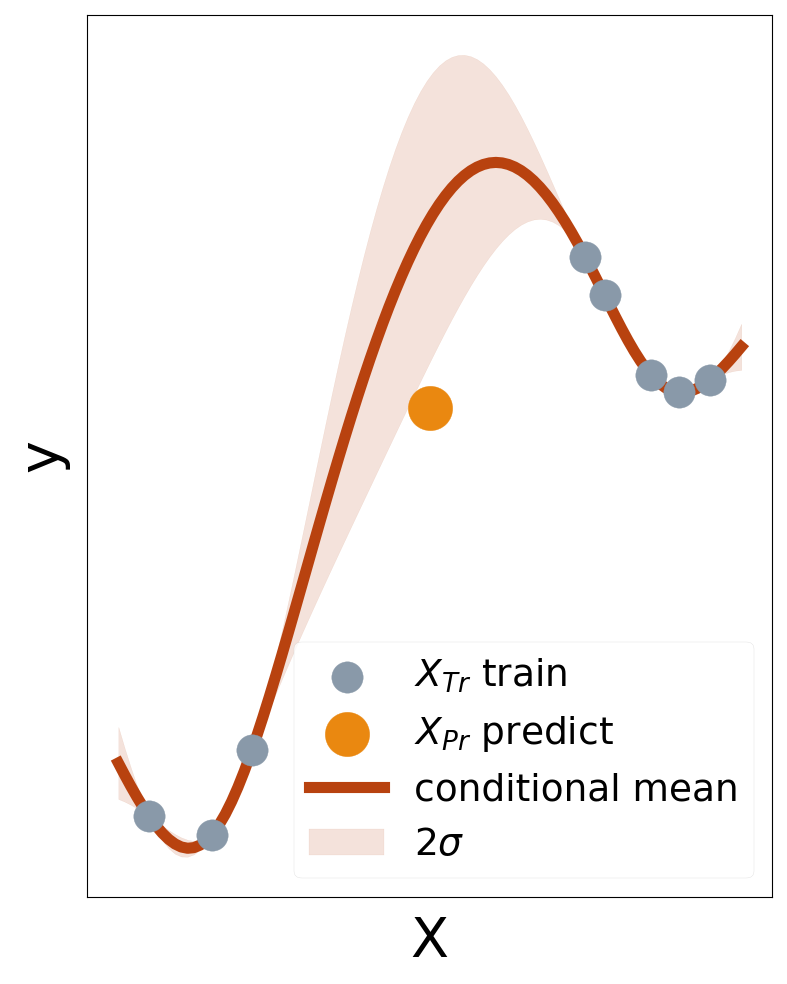
\includegraphics[width=\textwidth]{graphs/predict_all}
      \end{figure}
    \end{column}
  \end{columns}
\end{frame}

\begin{frame}
\frametitle{Conditional \( k \)-th Nearest Neighbors}
\framesubtitle{}

\begin{columns}
  \begin{column}{0.6\textwidth}
    \begin{itemize}
      \item<1-> Naive: select \( k \) closest points

      \item<2-> Chooses redundant information

      \item<3-> Maximize \emph{mutual information}!

      \item<5-> Direct computation: \( \mathcal{O}(N k^4) \)

      \item<6-> Store Cholesky factor \( \rightarrow \mathcal{O}(N k^2) \)!
    \end{itemize}
  \end{column}
  \begin{column}{0.4\textwidth}

    \only<1| handout:1>{
      \begin{figure}
        \centering
        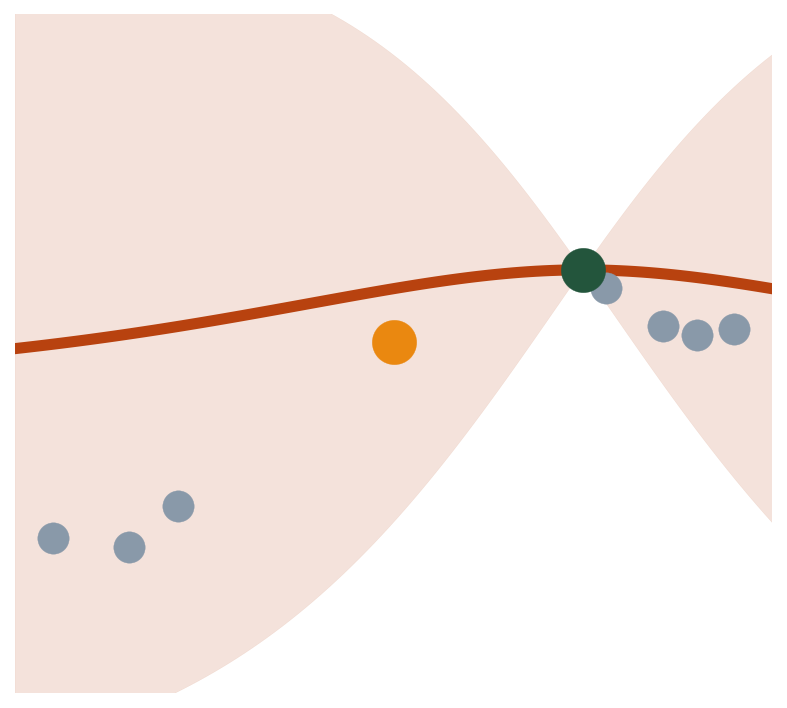
\includegraphics[width=\textwidth]{graphs/predict_knn_1}
      \end{figure}
    }

    \only<2- | handout:2->{
      \begin{figure}
        \centering
        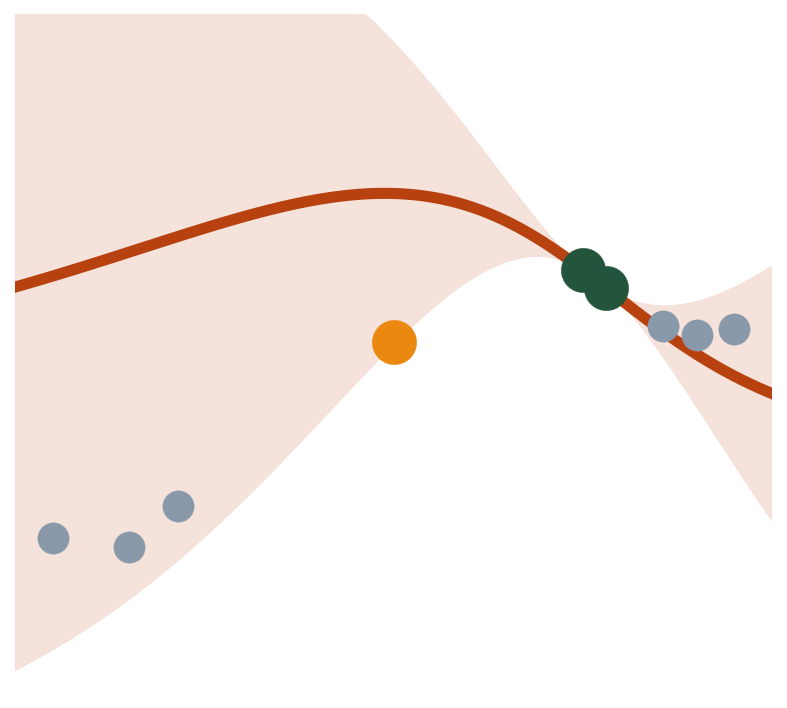
\includegraphics[width=\textwidth]{graphs/predict_knn_2}
      \end{figure}
    }

    \vspace{-0.6cm}

    \uncover<3- | handout:3-> {
      \only<-3 | handout:-3>{
        \begin{figure}
          \centering
          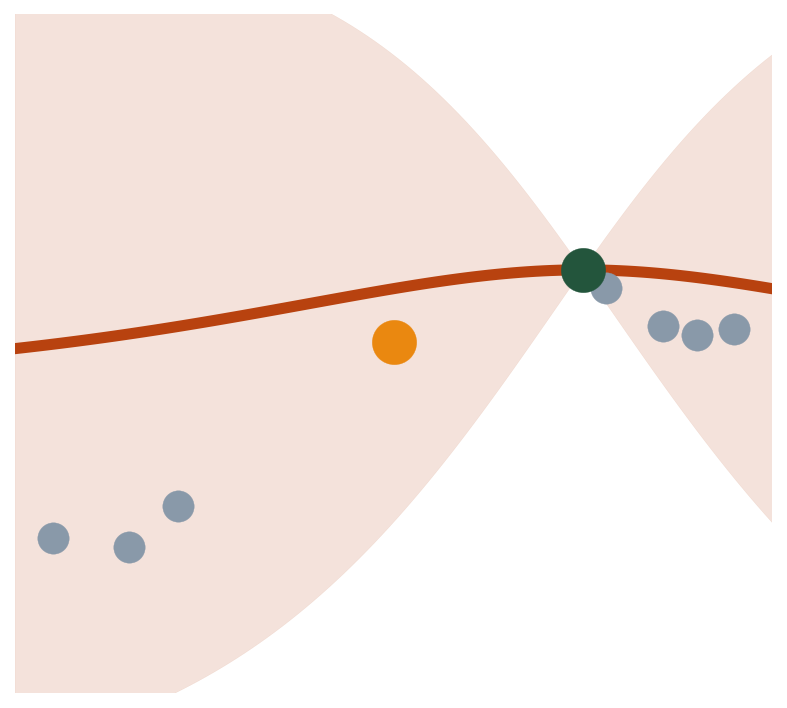
\includegraphics[width=\textwidth]{graphs/predict_cknn_1}
        \end{figure}
      }

      \only<4- | handout:4-> {
        \begin{figure}
          \centering
          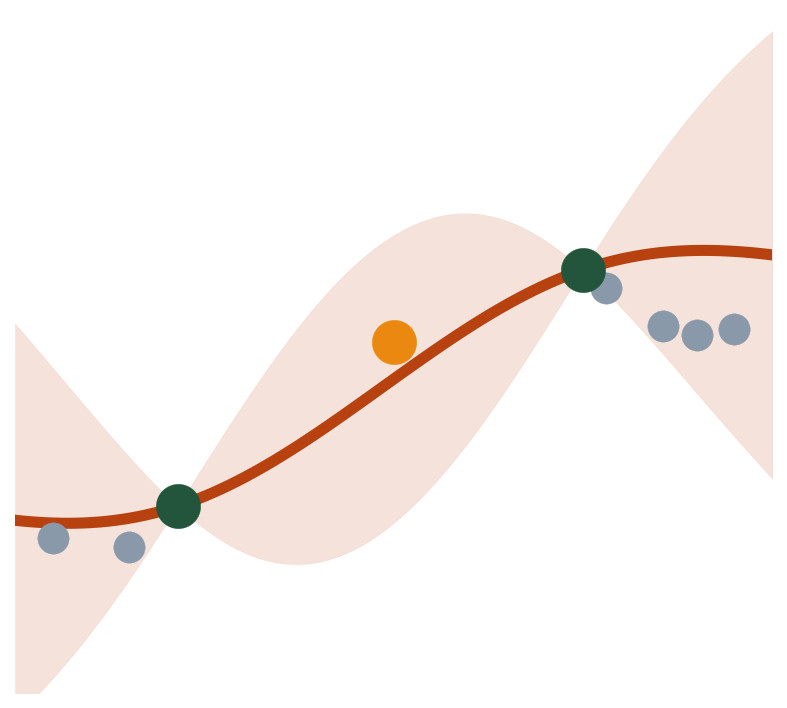
\includegraphics[width=\textwidth]{graphs/predict_cknn_2}
        \end{figure}
      }
    }

  \end{column}
\end{columns}

\end{frame}

% https://tex.stackexchange.com/questions/518750/beamer-how-to-make-footnote-rule-appear-later-pause
\begingroup
\let\oldfootnoterule\footnoterule
\renewcommand\footnoterule{\only<3->\oldfootnoterule}
\begin{frame}
\frametitle{Cholesky Factorization by Selection}
\framesubtitle{}

\begin{columns}
  \begin{column}{0.6\textwidth}
    \begin{itemize}
      \item<+-> Apply column-wise

        \( \rightarrow \) sparse approx. of GP

      \item<+-> Maximum mutual information

        \( \rightarrow \) minimum KL divergence

      \item<+-> Improves approx. algorithm of \footnotemark
    \end{itemize}
  \end{column}
  \begin{column}{0.4\textwidth}
    \begin{figure}[h!]
        \centering
        \begin{subfigure}[h]{\textwidth}
          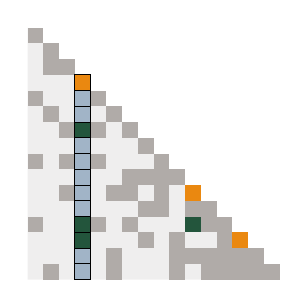
\begin{tikzpicture}[scale=1/5]
            % outer triangular factor
\fill[lightsilver] (0, 0) -- (0, -16) -- (16, -16) -- cycle;

% column rectangle
\draw[fill=lightblue] (3, -4) rectangle (4, -16);

% triangular factor
\fill[silver] (0, 0) rectangle (1, -1);
\fill[silver] (1, -1) rectangle (2, -2);
\fill[silver] (1, -2) rectangle (2, -3);
\fill[silver] (2, -2) rectangle (3, -3);
\fill[orange] (3, -3) rectangle (4, -4);
\draw (3, -3) rectangle (4, -4);
\fill[silver] (0, -4) rectangle (1, -5);
\draw (3, -4) rectangle (4, -5);
\fill[silver] (4, -4) rectangle (5, -5);
\fill[silver] (1, -5) rectangle (2, -6);
\draw (3, -5) rectangle (4, -6);
\fill[silver] (5, -5) rectangle (6, -6);
\fill[silver] (2, -6) rectangle (3, -7);
\fill[seagreen] (3, -6) rectangle (4, -7);
\draw (3, -6) rectangle (4, -7);
\fill[silver] (4, -6) rectangle (5, -7);
\fill[silver] (6, -6) rectangle (7, -7);
\draw (3, -7) rectangle (4, -8);
\fill[silver] (7, -7) rectangle (8, -8);
\fill[silver] (0, -8) rectangle (1, -9);
\fill[silver] (2, -8) rectangle (3, -9);
\draw (3, -8) rectangle (4, -9);
\fill[silver] (4, -8) rectangle (5, -9);
\fill[silver] (8, -8) rectangle (9, -9);
\draw (3, -9) rectangle (4, -10);
\fill[silver] (6, -9) rectangle (7, -10);
\fill[silver] (7, -9) rectangle (8, -10);
\fill[silver] (8, -9) rectangle (9, -10);
\fill[silver] (9, -9) rectangle (10, -10);
\fill[silver] (2, -10) rectangle (3, -11);
\draw (3, -10) rectangle (4, -11);
\fill[silver] (5, -10) rectangle (6, -11);
\fill[silver] (6, -10) rectangle (7, -11);
\fill[silver] (8, -10) rectangle (9, -11);
\fill[orange] (10, -10) rectangle (11, -11);
\draw (3, -11) rectangle (4, -12);
\fill[silver] (7, -11) rectangle (8, -12);
\fill[silver] (8, -11) rectangle (9, -12);
\fill[silver] (10, -11) rectangle (11, -12);
\fill[silver] (11, -11) rectangle (12, -12);
\fill[silver] (0, -12) rectangle (1, -13);
\fill[seagreen] (3, -12) rectangle (4, -13);
\draw (3, -12) rectangle (4, -13);
\fill[silver] (4, -12) rectangle (5, -13);
\fill[silver] (6, -12) rectangle (7, -13);
\fill[seagreen] (10, -12) rectangle (11, -13);
\fill[silver] (11, -12) rectangle (12, -13);
\fill[silver] (12, -12) rectangle (13, -13);
\fill[seagreen] (3, -13) rectangle (4, -14);
\draw (3, -13) rectangle (4, -14);
\fill[silver] (7, -13) rectangle (8, -14);
\fill[silver] (9, -13) rectangle (10, -14);
\fill[silver] (12, -13) rectangle (13, -14);
\fill[orange] (13, -13) rectangle (14, -14);
\draw (3, -14) rectangle (4, -15);
\fill[silver] (5, -14) rectangle (6, -15);
\fill[silver] (9, -14) rectangle (10, -15);
\fill[silver] (10, -14) rectangle (11, -15);
\fill[silver] (11, -14) rectangle (12, -15);
\fill[silver] (12, -14) rectangle (13, -15);
\fill[silver] (13, -14) rectangle (14, -15);
\fill[silver] (14, -14) rectangle (15, -15);
\fill[silver] (1, -15) rectangle (2, -16);
\draw (3, -15) rectangle (4, -16);
\fill[silver] (5, -15) rectangle (6, -16);
\fill[silver] (9, -15) rectangle (10, -16);
\fill[silver] (11, -15) rectangle (12, -16);
\fill[silver] (12, -15) rectangle (13, -16);
\fill[silver] (13, -15) rectangle (14, -16);
\fill[silver] (14, -15) rectangle (15, -16);
\fill[silver] (15, -15) rectangle (16, -16);

% column rectangle
\draw (3, -4) rectangle (4, -16);

          \end{tikzpicture}
        \end{subfigure}
        \begin{subfigure}[h]{0.4 \textwidth}
          \begin{tikzpicture}[overlay,remember picture]
            \node[below left=1.25cm and 1cm] at (current page.north east) {
                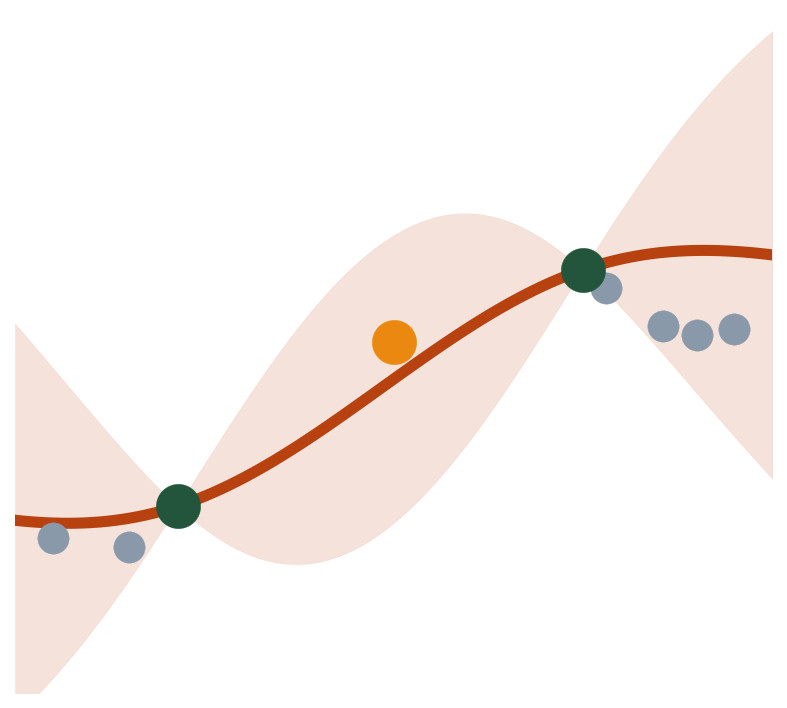
\includegraphics[width=2cm]{graphs/predict_cknn_2}
            };
          \end{tikzpicture}
        \end{subfigure}
    \end{figure}

    \vspace{-0.5cm}

    \begin{figure}[h!]
      \centering
      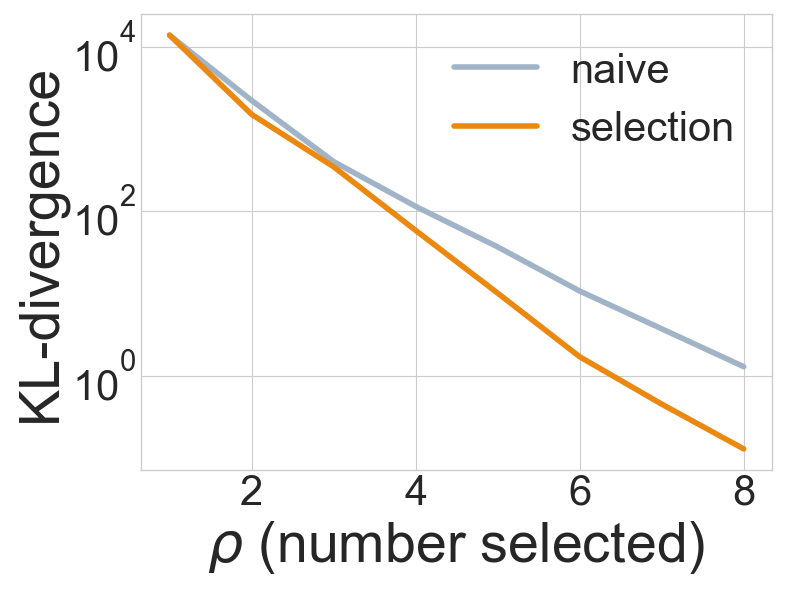
\includegraphics[width=\textwidth]{data/rho_kl-div}
    \end{figure}
  \end{column}
\end{columns}

% https://tex.stackexchange.com/questions/340058/uncovered-footnote-appears-too-early-in-beamer-presentation
\alt<3->{\footnotetext{\fullcite{schafer2020sparse}}}
{\let\thefootnote\relax\footnotetext{~ \newline ~}}
\end{frame}
\endgroup

\section{Cholesky Factorization}

\begin{frame}
\frametitle{LU Decomposition}
\framesubtitle{... and its symmetric counterpart}

\begin{itemize}
  \item<+-> \( M = LU \) where \( L \) is
    lower triangular and \( U \) is upper triangular
  \item<+-> Not always possible, need \( PLU \) in general!
  \item<+-> Special case for (square) symmetric matrices:
    \begin{theorem}
      If \( M = M^{\top} \) and \( \det(M) \neq 0 \), then \( M
      = L D L^T \) where \( L \) is from the LU decomposition
      of \( M \) and \( D \) is the diagonal of \( U \).
    \end{theorem}
    \uncover<3 | handout:0>{
      \begin{tikzpicture}[overlay,remember picture]
      \node[below right=0.1cm and 0cm] at (current page.north west) {
          
\includegraphics[width=3cm]{genshin/chibi/kokomi/06_chill.png}
      };
      \end{tikzpicture}
    }
  \item<+->
    \begin{proof}[Proof sketch.]
      (MATH3406 Fall 2021, Prof. Wing Li) Let \( M = LDK \). Just do
      matrix multiplication on \( M = M^{\top} \implies (LDK) = (LDK)^T \).
      From matrix multiplication, able to see \( K = L^{\top} \).
    \end{proof}
    \uncover<4 | handout:0>{
      \begin{tikzpicture}[overlay,remember picture]
      \node[below right=0.1cm and 0cm] at (current page.north west) {
          
\includegraphics[width=3cm]{genshin/chibi/kokomi/05_tired.png}
      };
      \end{tikzpicture}
    }
\end{itemize}
\end{frame}

\begin{frame}
\frametitle{Cholesky Factorization}
\framesubtitle{}
\begin{itemize}
  \item<+-> Let \( M \) be (symmetric) \emph{positive definite}.
  \item<+-> Then \( M = L D L^{\top} \) becomes \( L L^{\top} \):
    \begin{align*}
      M &= L D L^{\top} \\
        &= L D^{\frac{1}{2}} D^{\frac{1}{2}} L^{\top} \\
        &= L D^{\frac{1}{2}} (L D^{\frac{1}{2}})^{\top} \\
        &= L' L'^{\top}
    \end{align*}
    \uncover<2 | handout:0>{
      \begin{tikzpicture}[overlay,remember picture]
      \node[below right=0.1cm and 0cm] at (current page.north west) {
          
\includegraphics[width=3cm]{genshin/chibi/kokomi/07_catch_fish.png}
      };
      \end{tikzpicture}
    }
  \item<+-> This is the Cholesky factorization!
    \uncover<3 | handout:0>{
      \begin{tikzpicture}[overlay,remember picture]
      \node[below right=0.1cm and 0cm] at (current page.north west) {
          
\includegraphics[width=3cm]{genshin/chibi/kokomi/08_pray.png}
      };
      \end{tikzpicture}
    }
\end{itemize}
\end{frame}

\begin{frame}
\frametitle{Why Do We Care?}
\framesubtitle{}

\begin{itemize}
  \item \( \Theta = L L^{\top} \), \( L \) has \( N
    \) columns, \( s \) non-zero entries per column
  \item \( L \vec{v} \) and \( L^{-1} \vec{v} \)
    both cost \( \mathcal{O}(Ns) \)
  \item Matrix-vector product
    \( \Theta \vec{v} \rightarrow L (L^{\top} \vec{v}) \)
    \begin{itemize}
      \item \( N^2 \rightarrow Ns \)
    \end{itemize}
  \item Solving linear system
    \( \Theta^{-1} \vec{v} \rightarrow L^{-\top} (L^{-1} \vec{v}) \)
    \begin{itemize}
      \item \( N^3 \rightarrow Ns \)
    \end{itemize}
  \item Log determinant
    \( \logdet \Theta \rightarrow 2 \logdet L = 2 \sum_{i = 1}^N \log L_{ii} \)
    \begin{itemize}
      \item \( N^3 \rightarrow N \)
    \end{itemize}
  \item Sampling from
    \( \vec{x} \sim \mathcal{N}(\vec{\mu}, \Theta) \rightarrow
    \vec{z} \sim \mathcal{N}(\vec{0}, I), \vec{x} = L \vec{z} + \vec{\mu} \)
    \begin{itemize}
      \item \( \text{???} \rightarrow Ns \)
    \end{itemize}
\end{itemize}
\uncover<2 | handout:0>{
  \begin{tikzpicture}[overlay,remember picture]
  \node[above left=4cm and 0.5cm] at (current page.south east) {
      
\includegraphics[width=3cm]{genshin/chibi/sayu/10_angry.png}
  };
  \end{tikzpicture}
}
\end{frame}

\begin{frame}[fragile]
\frametitle{Computing the Cholesky Factorization}
\framesubtitle{Down-looking}
\begin{itemize}
  \item Like LU
  \item Gaussian elimination downwards
    \begin{minted}[fontsize=\small]{python}
def down_cholesky(theta: np.ndarray) -> np.ndarray:
    M, n = np.copy(theta), len(theta)
    L = np.identity(n)
    for i in range(n):
        for j in range(i + 1, n):
            L[j, i] = M[j, i]/M[i, i]
            # zero out everything below
            M[j] -= L[j, i]*M[i]
        # update L
        L[:, i] *= np.sqrt(M[i, i])
    return L
    \end{minted}
\end{itemize}
\uncover<2 | handout:0>{
  \begin{tikzpicture}[overlay,remember picture]
  \node[above left=4cm and 0.5cm] at (current page.south east) {
      
\includegraphics[width=3cm]{genshin/chibi/sayu/09_tired.png}
  };
  \end{tikzpicture}
}
\end{frame}

\begin{frame}
\frametitle{Computing the Cholesky Factorization}
\framesubtitle{Up-looking}
\vspace{-0.5cm}
\begin{align*}
  \shortintertext{Let \( L' \) be blocked according to:}
  L' &=
  \begin{pmatrix}
    L & \vec{0} \\
    \vec{r}^{\top} & d
  \end{pmatrix} \\
  L' L'^{\top} &=
  \begin{pmatrix}
    L & \vec{0} \\
    \vec{r}^{\top} & d
  \end{pmatrix}
  \begin{pmatrix}
    L^{\top} & \vec{r} \\
    \vec{0}^{\top} & d
  \end{pmatrix} \\
             &=
  \begin{pmatrix}
    L L^{\top} & L \vec{r} \\
    \vec{r}^{\top} L^{\top} & \vec{r}^{\top} \vec{r} + d^2
  \end{pmatrix}
  \shortintertext{So if we have a Cholesky factor for
    a principle submatrix of \( \Theta \), we can extend
    it inductively by reading off the appropiate data!}
  \begin{pmatrix}
    L L^{\top} & L \vec{r} \\
    \vec{r}^{\top} L^{\top} & \vec{r}^{\top} \vec{r} + d^2
  \end{pmatrix} &=
  \begin{pmatrix}
    \Theta & \vec{c} \\
    \vec{c}^{\top} & C
  \end{pmatrix} \\
  \vec{r} &= L^{-1} \vec{c} \\
  d &= \sqrt{C - \vec{r}^{\top} \vec{r}}
\end{align*}
{
\uncover<2 | handout:0>{
  \begin{tikzpicture}[overlay,remember picture]
  \node[above right=4cm and 1cm] at (current page.south west) {
      
\includegraphics[width=3cm]{genshin/chibi/sayu/12_alert.png}
  };
  \end{tikzpicture}
}
}
\end{frame}

\begin{frame}[fragile]
\frametitle{Computing the Cholesky Factorization}
\framesubtitle{Up-looking}
\begin{minted}[fontsize=\small]{python}
def Lsolve(L: np.ndarray, y: np.ndarray) -> np.ndarray:
    """ Solves Lx = y for lower triangular L. """
    n = len(y)
    x = np.zeros(n)
    for i in range(n):
        x[i] = (y[i] - L[i, :i].dot(x[:i]))/L[i, i]
    return x

def up_cholesky(theta: np.ndarray) -> np.ndarray:
    n = len(theta)
    L = np.zeros((n, n))
    for i in range(n):
        row = Lsolve(L, theta[:i, i])
        L[i, :i] = row
        L[i, i] = np.sqrt(theta[i, i] - row.dot(row))
    return L
\end{minted}
\uncover<2 | handout:0>{
  \begin{tikzpicture}[overlay,remember picture]
  \node[above right=4cm and 1cm] at (current page.south west) {
      
\includegraphics[width=3cm]{genshin/chibi/sayu/11_watch_me.png}
  };
  \end{tikzpicture}
}
\end{frame}

\begin{frame}
\frametitle{Computing the Cholesky Factorization}
\framesubtitle{Right-looking}
\begin{align*}
  L &=
  \begin{pmatrix}
    \vec{l}_1 & \vec{l}_2 & \cdots & \vec{l}_N
  \end{pmatrix} \\
  L L^{\top} &=
  \begin{pmatrix}
    \vec{l}_1 & \vec{l}_2 & \cdots & \vec{l}_N
  \end{pmatrix}
  \begin{pmatrix}
    \vec{l}_1^{\top} \\
    \vec{l}_2^{\top} \\
    \vdots \\
    \vec{l}_N^{\top}
  \end{pmatrix} \\
  &= \vec{l}_1 \vec{l}_1^{\top} + \vec{l}_2 \vec{l}_2^{\top} +
    \dotsb + \vec{l}_N \vec{l}_N^{\top} = \Theta
  \shortintertext{From lower triangularity, nested submatrices!}
\end{align*}
\uncover<2 | handout:0>{
  \begin{tikzpicture}[overlay,remember picture]
  \node[above right=4cm and 0.5cm] at (current page.south west) {
      
\includegraphics[width=3cm]{genshin/chibi/barbara/11_shhh.png}
  };
  \end{tikzpicture}
}
\end{frame}

\begin{frame}
\frametitle{Computing the Cholesky Factorization}
\framesubtitle{Right-looking}
\begin{align*}
  \vec{l}_1 \vec{l}_1^{\top} + \vec{l}_2 \vec{l}_2^{\top} +
  \dotsb + \vec{l}_N \vec{l}_N^{\top} &= \Theta \\
  \vec{l}_1 \vec{l}_1^{\top} &= \Theta_1 \\
  l_1^2 &= \Theta_{11} \\
  l_1 &= \sqrt{\Theta_{11}} \\
  \vec{l}_1 &= \frac{\Theta_1}{l_1} = \frac{\Theta_1}{\sqrt{\Theta_{11}}} \\
  \vec{l}_2 \vec{l}_2^{\top} + \dotsb + \vec{l}_N \vec{l}_N^{\top}
  &= \Theta - \left ( \frac{\Theta_1}{\sqrt{\Theta_{11}}} \right )
              \left ( \frac{\Theta_1}{\sqrt{\Theta_{11}}} \right )^{\top} \\
  &= \Theta - \frac{\Theta_1 \Theta_1^{\top}}{\Theta_{11}}
  \shortintertext{Proceed inductively on rank-one update}
\end{align*}
\uncover<2 | handout:0>{
  \begin{tikzpicture}[overlay,remember picture]
  \node[above right=3.5cm and 2cm] at (current page.south west) {
      
\includegraphics[width=3cm]{genshin/chibi/barbara/09_are_you_alright.png}
  };
  \end{tikzpicture}
}
\end{frame}

\begin{frame}[fragile]
\frametitle{Computing the Cholesky Factorization}
\framesubtitle{Right-looking}
\begin{minted}{python}
def right_cholesky(theta: np.ndarray) -> np.ndarray:
    M, n = np.copy(theta), len(theta)
    L = np.zeros((n, n))
    for i in range(n):
        L[:, i] = M[:, i]/np.sqrt(M[i, i])
        M -= np.outer(L[:, i], L[:, i])
    return L
\end{minted}
\end{frame}

\begin{frame}
\frametitle{Computing the Cholesky Factorization}
\framesubtitle{Left-looking}
\vspace{-0.2cm}
\begin{align*}
  \shortintertext{Recall:}
  \vec{l}_1 \vec{l}_1^{\top} + \vec{l}_2 \vec{l}_2^{\top} +
  \dotsb + \vec{l}_N \vec{l}_N^{\top} &= \Theta \\
  \shortintertext{Look at \( \vec{l}_i \):}
  \vec{l}_i \vec{l}_i^{\top}
  &= \left ( \Theta -
    (\vec{l}_1 \vec{l}_1^{\top} + \vec{l}_2 \vec{l}_2^{\top} + \dotsb +
     \vec{l}_{i - 1} \vec{l}_{i - 1}^{\top}) \right )_i \\
  &= \Theta_i - (l_{1i} \vec{l}_1 + l_{2i} \vec{l}_2 + \dotsb +
     l_{i - 1, i} \vec{l}_{i - 1}) \\
  &= \Theta_i -
  \begin{pmatrix}
    \vec{l}_1 & \vec{l}_2 & \cdots & \vec{l}_{i - 1}
  \end{pmatrix}
  \begin{pmatrix}
    l_{1i} \\
    l_{2i} \\
    \vdots \\
    l_{i, i - 1}
  \end{pmatrix} \\
  &= \Theta_i - L_{:, :i} L_{i, :i}
  \shortintertext{Don't need to store modified \( \Theta \) in memory!}
\end{align*}
\uncover<2 | handout:0>{
  \begin{tikzpicture}[overlay,remember picture]
  \node[above right=1.5cm and 0.5cm] at (current page.south west) {
      
\includegraphics[width=4cm]{genshin/chibi/barbara/12_panic.png}
  };
  \end{tikzpicture}
}
\end{frame}

\begin{frame}[fragile]
\frametitle{Computing the Cholesky Factorization}
\framesubtitle{Left-looking}
\begin{minted}{python}
def left_cholesky(theta: np.ndarray) -> np.ndarray:
    n = len(theta)
    L = np.zeros((n, n))
    for i in range(n):
        L[:, i] = theta[:, i] - L[:, :i]@L[i, :i]
        L[:, i] /= np.sqrt(L[i, i])
    return L
\end{minted}
\uncover<2 | handout:0>{
  \begin{tikzpicture}[overlay,remember picture]
  \node[above right=1.5cm and 0.5cm] at (current page.south west) {
      
\includegraphics[width=4cm]{genshin/chibi/barbara/10_shy.png}
  };
  \end{tikzpicture}
}
\end{frame}

\section{Schur Complement}

\begin{frame}
\frametitle{Schur Complement}
\framesubtitle{or recursive Cholesky factorization}
\vspace{-0.5cm}
\begin{align*}
\shortintertext{Block \( \Theta \) as follows:}
\Theta &=
\begin{pmatrix}
  \Theta_{11} & \Theta_{12} \\
  \Theta_{21} & \Theta_{22}
\end{pmatrix}
\shortintertext{Then proceed by one step of Gaussian elimination:}
       &
\begin{pmatrix}
  \Theta_{11} & \Theta_{12} \\
  \vec{0} & \Theta_{22} - \Theta_{21} \Theta_{11}^{-1} \Theta_{12}
\end{pmatrix}
\shortintertext{Thus,}
       &=
  \begin{pmatrix}
    I & 0 \\
    \textcolor{darkorange}{\Theta_{21} \Theta_{11}^{-1}} & I
  \end{pmatrix}
  \begin{pmatrix}
    \Theta_{11} & 0 \\
    0 & \textcolor{lightblue}{
      \Theta_{22} - \Theta_{21} \Theta_{11}^{-1} \Theta_{12}
    }
  \end{pmatrix}
  \begin{pmatrix}
    I & \textcolor{darkorange}{\Theta_{11}^{-1} \Theta_{12}} \\
    0 & I
  \end{pmatrix}
  \shortintertext{so we see the Cholesky factorization of \( \Theta \) is}
  &
  \begin{pmatrix}
    I & 0 \\
    \textcolor{darkorange}{\Theta_{21} \Theta_{11}^{-1}} & I
  \end{pmatrix}
  \begin{pmatrix}
    \chol(\Theta_{11}) & 0 \\
    0 & \chol(\textcolor{lightblue}{
      \Theta_{22} - \Theta_{21} \Theta_{11}^{-1} \Theta_{12}
    })
  \end{pmatrix} \\
  \shortintertext{The term in \textcolor{lightblue}{blue}
    is the \textcolor{lightblue}{\emph{Schur complement}}
    of \( \Theta \) on \( \Theta_{11} \)}
\end{align*}
\uncover<2 | handout:0>{
  \begin{tikzpicture}[overlay,remember picture]
  \node[below left=2cm and 0.5cm] at (current page.north east) {
      
\includegraphics[width=3cm]{genshin/chibi/eula/snowfall.png}
  };
  \end{tikzpicture}
}
\end{frame}

\begin{frame}
\frametitle{Proper Determinant of Block Matrix}
\framesubtitle{}
\begin{align*}
  \Theta &=
  \begin{pmatrix}
    \Theta_{11} & \Theta_{12} \\
    \Theta_{21} & \Theta_{22}
  \end{pmatrix} \\
  \det(\Theta) &= \text{?} \\
               &= \det(\Theta_{11}) \det(\Theta_{22}) -
                  \det(\Theta_{21}) \det(\Theta_{12})
               \text{?} && \text{wrong!} \\
               &= \det(\Theta_{11} \Theta_{22} - \Theta_{21} \Theta_{12})
               \text{?} && \text{wrong!} \\
  \shortintertext{Schur complement gives proper answer:}
  \Theta &=
  \begin{pmatrix}
    I & 0 \\
    \textcolor{darkorange}{\Theta_{21} \Theta_{11}^{-1}} & I
  \end{pmatrix}
  \hspace{-0.2cm}
  \begin{pmatrix}
    \Theta_{11} & 0 \\
    0 & \textcolor{lightblue}{
      \Theta_{22} - \Theta_{21} \Theta_{11}^{-1} \Theta_{12}
    }
  \end{pmatrix}
  &&
  \hspace{-0.55cm}
  \begin{pmatrix}
    I & \textcolor{darkorange}{\Theta_{11}^{-1} \Theta_{12}} \\
    0 & I
  \end{pmatrix} \\
  \det(\Theta) &= \det(\Theta_{11})
    \det(\textcolor{lightblue}{
      \Theta_{22} - \Theta_{21} \Theta_{11}^{-1} \Theta_{12}
    })
\end{align*}
\uncover<2 | handout:0>{
  \begin{tikzpicture}[overlay,remember picture]
  \node[above right=0.1cm and 2cm] at (current page.south west) {
      
\includegraphics[width=2.5cm]{genshin/chibi/eula/get_going.png}
  };
  \end{tikzpicture}
}
\end{frame}

\begin{frame}
\frametitle{Proper Submatrix of Inverse}
\framesubtitle{}
\begin{align*}
  \Theta &=
  \begin{pmatrix}
    \Theta_{11} & \Theta_{12} \\
    \Theta_{21} & \Theta_{22}
  \end{pmatrix} \\
  (\Theta^{-1})_{22} &= \text{?} \\
                     &= (\Theta_{22})^{-1} \text{?} && \text{wrong!}
  \shortintertext{Schur complement to the rescue again!}
\end{align*}
\end{frame}

\begin{frame}
\frametitle{Proper Submatrix of Inverse}
\framesubtitle{}
\begin{align*}
  \Theta &=
  \begin{pmatrix}
    I & 0 \\
    \textcolor{darkorange}{\Theta_{21} \Theta_{11}^{-1}} & I
  \end{pmatrix}
  \begin{pmatrix}
    \Theta_{11} & 0 \\
    0 & \textcolor{lightblue}{
      \Theta_{22} - \Theta_{21} \Theta_{11}^{-1} \Theta_{12}
    }
  \end{pmatrix}
  \begin{pmatrix}
    I & \textcolor{darkorange}{\Theta_{11}^{-1} \Theta_{12}} \\
    0 & I
  \end{pmatrix}
  \shortintertext{For notational convenience, we denote the Schur
    complement \textcolor{lightblue}{\( \Theta_{22} - \Theta_{21}
    \Theta_{11}^{-1} \Theta_{12} \)} as \textcolor{lightblue}{\(
    \Theta_{22 \mid 1} \)}. Inverting both sides of the equation,}
  \Theta^{-1} &=
  \begin{pmatrix}
    I & -\textcolor{darkorange}{\Theta_{11}^{-1} \Theta_{12}} \\
    0 & I
  \end{pmatrix}
  \begin{pmatrix}
    \Theta_{11}^{-1} & 0 \\
    0 & \textcolor{lightblue}{\Theta_{22 \mid 1}^{-1}}
  \end{pmatrix}
  \begin{pmatrix}
    I & 0 \\
    -\textcolor{darkorange}{\Theta_{21} \Theta_{11}^{-1}} & I
  \end{pmatrix} \\
  &=
  \begin{pmatrix}
    \Theta_{11}^{-1} +
    \textcolor{darkorange}{
      \left (\Theta_{11}^{-1} \Theta_{12} \right )
    } \textcolor{lightblue}{\Theta_{22 \mid 1}^{-1}}
    \textcolor{darkorange}{
      \left (\Theta_{21} \Theta_{11}^{-1} \right )
    } &
    - \textcolor{darkorange}{
      \left (\Theta_{11}^{-1} \Theta_{12} \right )
    } \textcolor{lightblue}{\Theta_{22 \mid 1}^{-1}} \\
    - \textcolor{lightblue}{\Theta_{22 \mid 1}^{-1}} \textcolor{darkorange} {
      \left (\Theta_{21} \Theta_{11}^{-1} \right )
    } & \textcolor{lightblue}{\Theta_{22 \mid 1}^{-1}}
  \end{pmatrix}
  \shortintertext{So \( (\Theta^{-1})_{22} \) can be read off as
    \( \Theta_{22 \mid 1}^{-1} \),}
  &= \left ( \textcolor{lightblue}{
    \Theta_{22} - \Theta_{21} \Theta_{11}^{-1} \Theta_{12}
  } \right )^{-1}
\end{align*}
\uncover<2 | handout:0>{
  \begin{tikzpicture}[overlay,remember picture]
  \node[above left=0.1cm and 4cm] at (current page.south east) {
      \scalebox{-1}[1]{
        
\includegraphics[width=2.5cm]{genshin/chibi/eula/get_going.png}
      }
  };
  \end{tikzpicture}
}
\end{frame}

\begin{frame}
\frametitle{A Few Important Questions...}
\framesubtitle{}

\begin{itemize}
  \item<+-> Is the Schur complement symmetric positive definite (s.p.d.)?
    \begin{itemize}
      \item<+-> If it isn't, we're kinda screwed
        --- have been assuming so
    \end{itemize}
  \item<+-> Is Schur complementing transitive?
    \begin{itemize}
      \item<+-> i.e. suppose we have \( \Theta \) blocked as
        \[
          \Theta =
          \begin{pmatrix}
            \Theta_{11} & \Theta_{12} & \Theta_{13} \\
            \Theta_{21} & \Theta_{22} & \Theta_{23} \\
            \Theta_{31} & \Theta_{32} & \Theta_{33}
          \end{pmatrix}
        \]
      \item<+-> Is \( \Theta \) complemented on \( \Theta_{11} \) and then
        on \( \Theta_{22} \) the same as \( \Theta \) complemented on
        \(
          \begin{pmatrix}
            \Theta_{11} & \Theta_{12} \\
            \Theta_{21} & \Theta_{22}
          \end{pmatrix}
        \)?
      \item<+-> Intuitively, it should be, but tedious to prove
        \uncover<6 | handout:0>{
          \begin{tikzpicture}[overlay,remember picture]
          \node[above left=4cm and 0.5cm] at (current page.south east) {
              
\includegraphics[width=3cm]{
                genshin/chibi/keqing/13_question.png
              }
          };
          \end{tikzpicture}
        }
    \end{itemize}
  \item<+-> New perspective which changes everything!
    \uncover<7 | handout:0>{
      \begin{tikzpicture}[overlay,remember picture]
      \node[above left=4cm and 0.5cm] at (current page.south east) {
          
\includegraphics[width=3cm]{
            genshin/chibi/keqing/14_congrats.png
          }
      };
      \end{tikzpicture}
    }
\end{itemize}

\end{frame}

\section{Multivariate Gaussians}

\begin{frame}
\frametitle{The Multivariate Gaussian}
\framesubtitle{}
\begin{itemize}
  \item<+-> Recall: Gaussian (or normal) distribution:
    \begin{align*}
      x &\sim \mathcal{N}(\mu, \sigma^2) \\
      f(x) &= \frac{1}{\sqrt{2 \pi \sigma^2}}
        e^{-\frac{1}{2} \frac{(x - \mu)^2}{\sigma^2}}
    \end{align*}
  \item<+-> Important (defining?) property: completely determined
    by mean and variance, all higher-order cumulants zero.
  \item<+-> We're going to extend this to higher dimensions. Consider
    \begin{align*}
      \vec{x} \sim \mathcal{N}(\vec{\mu}, \Sigma)
    \end{align*}
    where \( \vec{x} \) (\enquote{variables}) is a \( N \times 1 \) vector,
    \( \vec{\mu} \) (\enquote{mean vector}) is a \( N \times 1 \) vector, and
    \( \Sigma \) (\enquote{covariance matrix}) is a \( N \times N \) matrix
\end{itemize}
\end{frame}

\begin{frame}
\frametitle{Defining Everything}
\framesubtitle{}
\begin{itemize}
  \item<+-> Naturally,
    \begin{align*}
      \mu_i &= \E[x_i] \\
      \vec{\mu} &= \E[\vec{x}] \\
      \Sigma_{ij} &= \Cov[x_i, x_j] \\
                  &= \E[(x_i - \E[x_i])(x_j - \E[x_j])] \\
                  &= \E[(\vec{x} - \vec{\mu}) (\vec{x} - \vec{\mu})^{\top}]
    \end{align*}
  \item<+-> Two natural (and fundamental) questions from here:
    \begin{enumerate}
      \item What is the probability density function \( f(\vec{x}) \)?
      \item How can we sample from
        \( \vec{x} \sim \mathcal{N}(\vec{\mu}, \Sigma) \)?
    \end{enumerate}
  \item<+-> Surprisingly enough, Cholesky factorization answers both!
\end{itemize}
\uncover<4 | handout:0>{
  \begin{tikzpicture}[overlay,remember picture]
  \node[above right=4cm and 1cm] at (current page.south west) {
      
\includegraphics[width=2.5cm]{genshin/chibi/raiden/02_fly_away.png}
  };
  \end{tikzpicture}
}
\end{frame}

\begin{frame}
\frametitle{Independent Variables}
\framesubtitle{}
\begin{itemize}
  \item<+-> Gaussian has the (unique?) property if \(
    \Sigma_{ij} = 0 \), then \( x_i \) and \( x_j \) are
    statistically independent. This is not true in general!
  \item<+-> Key property we will make heavy use of: moment matching.
    If we know \( \vec{\mu} \) and \( \Sigma \), distribution is determined.
  \item<+-> Consider: if \( x_i \) and \( x_j \) \emph{were} independent,
    then \( \Sigma_{ij} = 0 \). So suppose \( x_i \) and \( x_j \) are not
    independent but \( \Sigma_{ij} = 0 \). It's the same \( \Sigma \) as when
    they were independent. So \( x_i \) and \( x_j \) must be distributed like
    they're independent. By contradiction, they must have been independent in
    the first place!
\end{itemize}
\uncover<4 | handout:0>{
  \begin{tikzpicture}[overlay,remember picture]
  \node[above left=0.1cm and 1cm] at (current page.south east) {
      
\includegraphics[width=2cm]{genshin/chibi/raiden/04_threaten.png}
  };
  \end{tikzpicture}
}
\end{frame}

\begin{frame}
\frametitle{Completely Independent Variables}
\framesubtitle{}
\begin{align*}
  \shortintertext{Well, if \( \Sigma \) has particular structure,
    it's actually trivial:}
  \vec{z} &\sim \mathcal{N}(\vec{0}, I_N) \\
  z_i &\overset{\text{i.i.d.}}{\sim} \mathcal{N}(0, 1) \\
  f(\vec{z})
  &= \prod_{i = 1}^N f(z_i) \\
  &= \prod_{i = 1}^N \frac{1}{\sqrt{2 \pi}} e^{-\frac{1}{2} z_i^2} \\
  &= \frac{1}{\sqrt{(2 \pi)^N}}
    e^{-\frac{1}{2} (z_1^2 + z_2^2 + \dotsb + z_N^2)} \\
  &= \frac{1}{\sqrt{(2 \pi)^N}} e^{-\frac{1}{2} \vec{z}^{\top} \vec{z}}
\end{align*}
\uncover<2 | handout:0>{
  \begin{tikzpicture}[overlay,remember picture]
  \node[above left=3cm and 2cm] at (current page.south east) {
      
\includegraphics[width=3cm]{genshin/chibi/raiden/01_chuckle.png}
  };
  \end{tikzpicture}
}
\end{frame}

\begin{frame}
\frametitle{Moment Matching}
\framesubtitle{}
\begin{itemize}
  \item How can we generalize to arbitrary \( \Sigma \)?
  \item Moment match!
  \begin{align*}
    \vec{z} &\sim \mathcal{N}(\vec{0}, I_N) \\
    \vec{x} &= L \vec{z} + \vec{\mu} \\
    \E[\vec{x}] &= \E[L \vec{z} + \vec{\mu}]
      = L \E[\vec{z}] + \vec{\mu} = \vec{\mu} \\
    \Cov[\vec{x}]
    &= \E[(\vec{x} - \E[\vec{x}]) (\vec{x} - \E[\vec{x}])^{\top}] \\
    &= \E[L \vec{z} (L \vec{z})^{\top}] \\
    &= \E[L \vec{z} \vec{z}^{\top} L^{\top}] \\
    &= L \E[\vec{z} \vec{z}^{\top}] L^{\top} \\
    &= L L^{\top}
    \shortintertext{so \( \vec{x} \sim \mathcal{N}(\vec{\mu}, L
      L^{\top}) \). We want \( \vec{x} \sim \mathcal{N}(\vec{\mu},
      \Sigma) \), so \( \Sigma = L L^{\top} \)}
  \end{align*}
\end{itemize}
\uncover<2 | handout:0>{
  \begin{tikzpicture}[overlay,remember picture]
  \node[below left=1cm and 1cm] at (current page.north east) {
      
\includegraphics[width=3cm]{genshin/chibi/raiden/03_yum.png}
  };
  \end{tikzpicture}
}
\end{frame}

\begin{frame}
\frametitle{Sampling with Cholesky Factorization}
\framesubtitle{}
\begin{itemize}
  \item<+-> As we just saw, we can sample
    \( \vec{x} \sim \mathcal{N}(\vec{\mu}, \Sigma) \) by instead sampling
    \( \vec{z} \sim \mathcal{N}(\vec{0}, I_N) \) and computing
    \( \vec{x} = L \vec{z} + \vec{\mu} \).
  \item<+-> Since \( L L^{\top} = \Sigma \), a natural pick is
    \( L = \chol(\Sigma) \).
  \item<+-> Why is \( \Sigma \) s.p.d.? Because it's a covariance/Gram matrix!
    \begin{align*}
      \Sigma &= \E[(\vec{x} - \vec{\mu}) (\vec{x} - \vec{\mu})^{\top}] \\
      \vec{y}^{\top} \Sigma \vec{y}
      &= \vec{y}^{\top} \E[(\vec{x} - \vec{\mu})
                           (\vec{x} - \vec{\mu})^{\top}] \vec{y} \\
      &= \E[\vec{y}^{\top} (\vec{x} - \vec{\mu})
                           (\vec{x} - \vec{\mu})^{\top} \vec{y}] \\
      &= \E[((\vec{x} - \vec{\mu})^{\top} \vec{y})^{\top}
             (\vec{x} - \vec{\mu})^{\top} \vec{y}] \\
      &= \E[\lVert (\vec{x} - \vec{\mu})^{\top} \vec{y} \rVert^2] \geq 0
    \end{align*}
\end{itemize}
\uncover<4 | handout:0>{
  \begin{tikzpicture}[overlay,remember picture]
  \node[above right=0.1cm and 0cm] at (current page.south west) {
      
\includegraphics[width=3.5cm]{
        genshin/chibi/ayaka/01_ayaka_chuckle.png
      }
  };
  \end{tikzpicture}
}
\end{frame}

\begin{frame}
\frametitle{Probability Density Function from Sampling}
\framesubtitle{}
\begin{itemize}
  \item<+-> What's the probability density function \( f(\vec{x}) \)?
  \item<+-> Idea: view \( \vec{x} \) resulting from
    a invertible transformation from \( \vec{z} \).
  \item<+-> We know \( f(\vec{z}) \), so \( f(\vec{x}) \) should be similar!
  \item<+-> In scalars:
    \begin{align*}
      z &\sim \mathcal{N}(0, 1) \\
      x &= \sigma z + \mu \\
      x &\sim \mathcal{N}(\mu, \sigma^2) \\
      z &= \frac{x - \mu}{\sigma}
    \end{align*}
\end{itemize}
\end{frame}

\begin{frame}
\frametitle{PDF from Sampling --- Scalar Edition}
\framesubtitle{}
\begin{align*}
  \shortintertext{Since \( f(z) \) is a valid probability density function,}
  1 &= \int_{-\infty}^\infty f(z) \D z
     = \int_{-\infty}^\infty f(z) \frac{\mathrm{d} z}{\mathrm{d} x} \D x
  \shortintertext{We now perform the change of variables
    \( z = \frac{x - \mu}{\sigma} \)}
  &= \int_{-\infty}^\infty
  \underbrace{f \left ( \frac{x - \mu}{\sigma} \right ) \frac{1}{\sigma}}_{
    \text{PDF of \( x \)}} \D x \\
  f(z) &= \frac{1}{\sqrt{2 \pi}} e^{-\frac{1}{2} z^2} \\
  \frac{1}{\sigma} f \left ( \frac{x - \mu}{\sigma} \right )
  &= \frac{1}{\sigma} \frac{1}{\sqrt{2 \pi}}
    e^{-\frac{1}{2} \left ( \frac{x - \mu}{\sigma} \right )^2} \\
  &= \frac{1}{\sqrt{2 \pi \sigma^2}}
    e^{-\frac{1}{2} \frac{(x - \mu)^2}{\sigma^2}}
\end{align*}
\end{frame}

\begin{frame}
\frametitle{PDF from Sampling --- Vector Edition}
\framesubtitle{}
\begin{align*}
  \vec{x} &= L \vec{z} + \vec{\mu} \\
  \vec{z} &= L^{-1} (\vec{x} - \vec{\mu}) \\
  \shortintertext{Since \( f(\vec{z}) \)
    is a valid probability density function,}
  1 &= \int_{-\infty}^\infty \dotsi \int_{-\infty}^\infty
    f(\vec{z}) \D \vec{z} \\
    &= \int_{-\infty}^\infty \dotsi \int_{-\infty}^\infty
    f(\vec{z}) \frac{\mathrm{d} \vec{z}}{\mathrm{d} \vec{x}} \D \vec{x}
    && \text{(informal)} \\
    &= \int_{-\infty}^\infty \dotsi \int_{-\infty}^\infty
    f(\vec{z}) \lvert \det(J_{\vec{z}}) \rvert \D \vec{x}
    && \text{(formal)} \\
    &= \int_{-\infty}^\infty \dotsi \int_{-\infty}^\infty
    \underbrace{f(L^{-1} (\vec{x} - \vec{\mu})) \det(L^{-1})}_{
      \text{PDF of \( \vec{x} \)}
    } \D \vec{x}
\end{align*}
\end{frame}

\begin{frame}
\frametitle{PDF from Sampling --- Vector Edition}
\framesubtitle{}
\begin{align*}
  f(\vec{z}) &= \frac{1}{\sqrt{(2 \pi)^N}}
    e^{-\frac{1}{2} \vec{z}^{\top} \vec{z}} \\
  \shortintertext{Expanding
    \( \det(L^{-1}) f(L^{-1} (\vec{x} - \vec{\mu})) \),}
  &= \frac{1}{\det(L)} f(L^{-1} (\vec{x} - \vec{\mu})) \\
  &= \frac{1}{\det(L)} \frac{1}{\sqrt{(2 \pi)^N}}
    e^{-\frac{1}{2} (L^{-1} (\vec{x} - \vec{\mu}))^{\top}
                    (L^{-1} (\vec{x} - \vec{\mu}))}
  \shortintertext{Since \( L L^{\top} = \Sigma \),
    \( \det(\Sigma) = \det(L)^2 \)}
  &= \frac{1}{\sqrt{(2 \pi)^N \det(\Sigma)}}
    e^{-\frac{1}{2} (\vec{x} - \vec{\mu})^{\top} L^{-T}
                     L^{-1} (\vec{x} - \vec{\mu})} \\
  &= \frac{1}{\sqrt{(2 \pi)^N \det(\Sigma)}}
    e^{-\frac{1}{2} (\vec{x} - \vec{\mu})^{\top} \Sigma^{-1}
                    (\vec{x} - \vec{\mu})}
\end{align*}
\uncover<2 | handout:0>{
  \begin{tikzpicture}[overlay,remember picture]
  \node[below left=1.5cm and 2cm] at (current page.north east) {
      
\includegraphics[width=3cm]{genshin/chibi/xiangling/16_ehehe.png}
  };
  \end{tikzpicture}
}
\end{frame}

\begin{frame}
\frametitle{Summary}
\framesubtitle{}
\begin{itemize}
  \item<+-> Compare PDFs of multivariate normal and scalar normal:
    \begin{align*}
      \vec{x} &\sim \mathcal{N}(\vec{\mu}, \Sigma) \\
      f(\vec{x}) &= \frac{1}{\sqrt{(2 \pi)^N \det(\Sigma)}}
        e^{-\frac{1}{2} (\vec{x} - \vec{\mu})^{\top} \Sigma^{-1}
                        (\vec{x} - \vec{\mu})}
      \shortintertext{Compare to scalar:}
      x &\sim \mathcal{N}(\mu, \sigma^2) \\
      f(x) &= \frac{1}{\sqrt{2 \pi \sigma^2}}
        e^{-\frac{1}{2} \frac{(x - \mu)^2}{\sigma^2}}
    \end{align*}
  \item<+-> Remarkable similarity!
    \uncover<2 | handout:0>{
      \begin{tikzpicture}[overlay,remember picture]
      \node[above left=0.1cm and 0cm] at (current page.south east) {
          
\includegraphics[width=4cm]{genshin/chibi/xiangling/15_excited.png}
      };
      \end{tikzpicture}
    }
\end{itemize}
\end{frame}

\begin{frame}
\frametitle{Cholesky Factorization for Gaussians}
\framesubtitle{}
\begin{itemize}
  \item Sampling: \( \vec{x} = L \vec{z} + \mu \),
    matrix-vector product, \( \mathcal{O}(Ns) \)
  \item Density computation:
    \begin{align*}
      (\vec{x} - \vec{\mu})^{\top} \Sigma^{-1} (\vec{x} - \vec{\mu})
      &= (\vec{x} - \vec{\mu})^{\top} L^{-\top} L^{-1} (\vec{x} - \vec{\mu}) \\
      &= (L^{-1} (\vec{x} - \vec{\mu}))^{\top} L^{-1} (\vec{x} - \vec{\mu}) \\
      &= \lVert L^{-1} (\vec{x} - \vec{\mu}) \rVert^2
    \end{align*}
    Back-substitution, \( O(Ns) \)
\end{itemize}
\uncover<2 | handout:0>{
  \begin{tikzpicture}[overlay,remember picture]
  \node[above left=0.1cm and 1cm] at (current page.south east) {
      
\includegraphics[width=3cm]{genshin/chibi/jean/14_angry.png}
  };
  \end{tikzpicture}
}
\end{frame}

\begin{frame}
\frametitle{Closure of Multivariate Gaussians}
\framesubtitle{}
\begin{itemize}
  \item<+-> Many statistical operations preserve distribution
  \item<+-> Affine transformation
  \item<+-> Joint distribution \& marginalization:
    \begin{align*}
      \vec{x}_1 &\sim \mathcal{N}(\vec{\mu}_1, \Sigma_{11}) \\
      \vec{x}_2 &\sim \mathcal{N}(\vec{\mu}_2, \Sigma_{22}) \\
      \begin{pmatrix}
        \vec{x}_1 \\
        \vec{x}_2
      \end{pmatrix}
      &\sim
      \mathcal{N} \left (
      \begin{pmatrix}
        \vec{\mu}_1 \\
        \vec{\mu}_2
      \end{pmatrix},
      \begin{pmatrix}
        \Sigma_{11} & \Sigma_{12} \\
        \Sigma_{21} & \Sigma_{22}
      \end{pmatrix} \right )
    \end{align*}
  \item<+-> Conditioning
\end{itemize}
\uncover<5 | handout:0>{
  \begin{tikzpicture}[overlay,remember picture]
  \node[above left=3.5cm and 0cm] at (current page.south east) {
      
\includegraphics[width=4cm]{genshin/chibi/jean/16_ponder.png}
  };
  \end{tikzpicture}
}
\end{frame}

\begin{frame}
\frametitle{Conditioning}
\framesubtitle{}
\begin{align*}
  \shortintertext{Assume \( \vec{\mu} = \vec{0} \)
    and use precision instead of covariance!}
  Q &= \Sigma^{-1}
     =
  \begin{pmatrix}
    Q_{11} & Q_{12} \\
    Q_{21} & Q_{22} \\
  \end{pmatrix} \\
  \pi(\vec{x}_2 \mid \vec{x}_1) &=
    \frac{\pi(\vec{x}_1 \mid \vec{x}_2) \pi(\vec{x}_2)}{\pi(\vec{x}_1)} =
    \frac{\pi(\vec{x}_1, \vec{x}_2)}{\pi(\vec{x}_1)} \\
  &\propto \pi(\vec{x}_1, \vec{x}_2) \\
  &\propto e^{-\frac{1}{2} \vec{x}_2^{\top} Q_{22} \vec{x}_2 -
    (Q_{21} \vec{x}_1 )^{\top} \vec{x}_2} \\
  \vec{x}_2 \mid \vec{x}_1 &\sim \mathcal{N} \left (-Q_{22}^{-1} Q_{21} \vec{x}_1,
    Q_{22}^{-1} \right )
  \shortintertext{If \( \vec{\mu} \neq \vec{0} \), shift
    \( \vec{x}^* = \vec{x} - \vec{\mu} \), \( \E[\vec{x}^*] = \vec{0} \)}
  \vec{x}_2 \mid \vec{x}_1 &\sim \mathcal{N} \left (
    \vec{\mu}_2 - Q_{22}^{-1} Q_{21} (\vec{x}_1 - \vec{\mu}_1),
    Q_{22}^{-1}
  \right )
\end{align*}
\end{frame}

\begin{frame}
\frametitle{Conditioning with Schur Complements}
\framesubtitle{}
\begin{align*}
  \vec{x}_2 \mid \vec{x}_1 &\sim \mathcal{N} \left (
    \vec{\mu}_2 - Q_{22}^{-1} Q_{21} (\vec{x}_1 - \vec{\mu}_1),
    Q_{22}^{-1}
  \right ) \\
  Q &= \Sigma^{-1}
     =
  \begin{pmatrix}
    Q_{11} & Q_{12} \\
    Q_{21} & Q_{22} \\
  \end{pmatrix} \\
    &=
  \begin{pmatrix}
    \Sigma_{11}^{-1} +
    \textcolor{darkorange}{
      \left (\Sigma_{11}^{-1} \Sigma_{12} \right )
    } \textcolor{lightblue}{\Sigma_{22 \mid 1}^{-1}}
    \textcolor{darkorange}{
      \left (\Sigma_{21} \Sigma_{11}^{-1} \right )
    } &
    - \textcolor{darkorange}{
      \left (\Sigma_{11}^{-1} \Sigma_{12} \right )
    } \textcolor{lightblue}{\Sigma_{22 \mid 1}^{-1}} \\
    - \textcolor{lightblue}{\Sigma_{22 \mid 1}^{-1}} \textcolor{darkorange} {
      \left (\Sigma_{21} \Sigma_{11}^{-1} \right )
    } & \textcolor{lightblue}{\Sigma_{22 \mid 1}^{-1}}
  \end{pmatrix} \\
  Q_{22}^{-1} &= (\Sigma_{22 \mid 1}^{-1})^{-1} = \Sigma_{22 \mid 1} \\
              &= \Sigma_{22} - \Sigma_{21} \Sigma_{11}^{-1} \Sigma_{12} \\
  Q_{22}^{-1} Q_{21} &= -\Sigma_{22 \mid 1}
  (\Sigma_{22 \mid 1}^{-1} \Sigma_{21} \Sigma_{11}^{-1}) \\
                     &= -\Sigma_{21} \Sigma_{11}^{-1} \\
  \vec{x}_2 \mid \vec{x}_1 &\sim \mathcal{N} \left (
    \vec{\mu}_2 + \Sigma_{21} \Sigma_{11}^{-1} (\vec{x}_1 - \vec{\mu}_1),
    \Sigma_{22} - \Sigma_{21} \Sigma_{11}^{-1} \Sigma_{12}
  \right )
\end{align*}
\uncover<2 | handout:0>{
  \begin{tikzpicture}[overlay,remember picture]
  \node[above left=1.5cm and 3cm] at (current page.south east) {
      
\includegraphics[width=3cm]{genshin/chibi/hu-tao/06_aloha.png}
  };
  \end{tikzpicture}
}
\end{frame}

\begin{frame}
\frametitle{Statistical Interpretation}
\framesubtitle{}
\begin{itemize}
  \item<+-> From conditioning,
    \[
      \vec{x}_2 \mid \vec{x}_1 \sim \mathcal{N} \left (
        \textcolor{darkorange}{
          \vec{\mu}_2 + \Sigma_{21} \Sigma_{11}^{-1}
        }(\vec{x}_1 - \vec{\mu}_1),
        \textcolor{lightblue}{
          \Sigma_{22} - \Sigma_{21} \Sigma_{11}^{-1} \Sigma_{12}
        }
      \right )
    \]
  \item<+-> Schur complement \( \iff \) conditional covariance!
  \item<+-> s.p.d. because covariance matrices s.p.d.
  \item<+-> Quotient rule statistically trivial:
    \( \pi((x_1 \mid x_2) \mid x_3) = \pi(x_1 \mid x_2, x_3) \)
  \item<+-> Conditioning in covariance \( \iff \) marginalization in precision
\end{itemize}
\uncover<6 | handout:0>{
  \begin{tikzpicture}[overlay,remember picture]
  \node[above left=2cm and 0cm] at (current page.south east) {
    
\includegraphics[width=3cm]{genshin/chibi/ayaka/02_drink_tea.png}
  };
  \end{tikzpicture}
}
\end{frame}

\section{Gaussian Process Regression}

\begin{frame}
\frametitle{Gaussian Processes}
\framesubtitle{}
\begin{itemize}
  \item<+-> Probability distribution over \emph{vectors}
  \item<+-> Extend to distribution over \emph{functions}?
  \item<+-> Idea: for finite set of points, function simply vector
    \begin{align*}
      % \vec{x} &=
      % \begin{pmatrix}
      % x_1 \\
      % x_2 \\
      % \vdots \\
      % x_N
      % \end{pmatrix}, \;
      % \vec{y} = f(\vec{x}) =
      % \begin{pmatrix}
      % f(x_1) \\
      % f(x_2) \\
      % \vdots \\
      % f(x_N)
      % \end{pmatrix} \\
      X &= \{ \vec{x}_1, \vec{x}_2, \dotsc, \vec{x}_N \} \\
      \vec{y} &= \{ f(\vec{x}_1), f(\vec{x}_2), \dotsc, f(\vec{x}_N) \}
    \end{align*}
  \item<+-> Idea: for points we're not given, marginalization is trivial
  \item<+-> How to assign mean and covariance in a sensible way?
\end{itemize}
\uncover<6 | handout:0>{
  \begin{tikzpicture}[overlay,remember picture]
  \node[below left=1cm and 0cm] at (current page.north east) {
      
\includegraphics[width=3cm]{genshin/chibi/ayaka/04_good_morning.png}
  };
  \end{tikzpicture}
}
\end{frame}

\begin{frame}
\frametitle{Gaussian Process Definition}
\framesubtitle{}
\begin{itemize}
  \item Let \( \mu(\vec{x}) \) be the \emph{mean function} and

    \( K(\vec{x}, \vec{x}') \) be the \emph{covariance
    function} or \emph{kernel function}
  \item We say
    \begin{align*}
      f(\vec{x}) &\sim \mathcal{GP}(\mu(\vec{x}), K(\vec{x}, \vec{x}'))
      \shortintertext{If for all point sets \( X \),}
      X &= \{ \vec{x}_1, \vec{x}_2, \dotsc, \vec{x}_N \} \\
      \vec{y} &= \{ f(\vec{x}_1), f(\vec{x}_2), \dotsc, f(\vec{x}_N) \} \\
      \vec{y} &\sim \mathcal{N}(\vec{\mu}, \Theta)
      \shortintertext{where}
      \vec{\mu}_i &= \mu(\vec{x}_i) \\
      \Theta_{ij} &= K(\vec{x}_i, \vec{x}_j)
    \end{align*}
\end{itemize}
\end{frame}

\begin{frame}
\frametitle{Regression with Gaussian Processes}
\framesubtitle{}
\begin{itemize}
  \item<+-> Simply condition prediction points on training points:
    \begin{align*}
      \Theta &=
      \begin{pmatrix}
        \Theta_{\text{Tr}, \text{Tr}} & \Theta_{\text{Tr}, \text{Pr}} \\
        \Theta_{\text{Pr}, \text{Tr}} & \Theta_{\text{Pr}, \text{Pr}}
      \end{pmatrix} \\
      \E[\vec{y}_\text{Pr} \mid \vec{y}_\text{Tr}] &=
        \vec{\mu}_\text{Pr} +
        \Theta_{\text{Pr}, \text{Tr}} \Theta_{\text{Tr}, \text{Tr}}^{-1}
        (\vec{y}_\text{Tr} - \vec{\mu}_\text{Tr}) \\
      \Cov[\vec{y}_\text{Pr} \mid \vec{y}_\text{Tr}] &=
        \Theta_{\text{Pr}, \text{Pr}} -
        \Theta_{\text{Pr}, \text{Tr}} \Theta_{\text{Tr}, \text{Tr}}^{-1}
        \Theta_{\text{Tr}, \text{Pr}}
    \end{align*}
  \item<+-> Nonparametric! No training! Uncertainty quantification!
    \uncover<2 | handout:0>{
      \begin{tikzpicture}[overlay,remember picture]
      \node[above left=0.1cm and 0cm] at (current page.south east) {
          
\includegraphics[width=3cm]{figures/genshin/chibi/klee/03_yay.png}
      };
      \end{tikzpicture}
    }
  \item<+-> ... \( \mathcal{O}(N^3) \) to compute
    \( \Theta_{\text{Tr}, \text{Tr}}^{-1} \)
    \uncover<3 | handout:0>{
      \begin{tikzpicture}[overlay,remember picture]
      \node[above left=0.1cm and 0cm] at (current page.south east) {
          
\includegraphics[width=3cm]{figures/genshin/chibi/klee/04_sad.png}
      };
      \end{tikzpicture}
    }
  \item<+-> And we're back to the starting problem
    \uncover<4 | handout:0>{
      \begin{tikzpicture}[overlay,remember picture]
      \node[above left=0.1cm and 0cm] at (current page.south east) {
          
\includegraphics[width=3cm]{genshin/chibi/klee/01_come_and_play.png}
      };
      \end{tikzpicture}
    }
\end{itemize}
\end{frame}

\begin{frame}
\frametitle{Screening Effect}
\framesubtitle{}
\begin{figure}[h!]
  \centering
  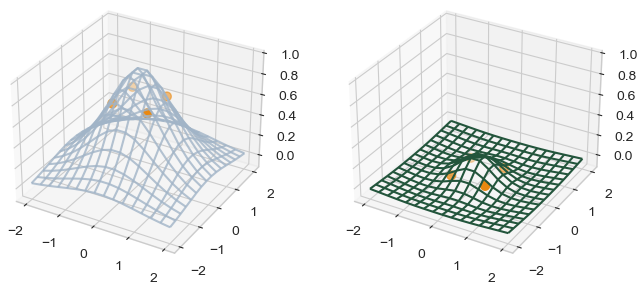
\includegraphics[width=\textwidth]{kernel2d.png}
  \caption{Conditional on nearby points, far away points have less covariance}
\end{figure}
\end{frame}

\section{Sparse Cholesky Factorization}

\begin{frame}
\frametitle{Cholesky Factorization by KL Minimization}
\framesubtitle{}
\begin{itemize}
  \item<+-> Measure approximation error by KL divergence:
    \begin{align*}
      L \coloneqq \argmin_{\hat{L} \in S} \, \mathbb{D}_{\text{KL}} \left (
        \mathcal{N}(\vec{0}, \Theta) \, \Big \| \,
        \mathcal{N}(\vec{0}, (\hat{L} \hat{L}^{\top})^{-1})
      \right )
    \end{align*}
  \item<+-> Re-write KL divergence:
    \begin{align*}
      & 2 \mathbb{D}_{\text{KL}}
      \left (
        \mathcal{N}(\vec{0}, \Theta_1) \, \Big \| \,
        \mathcal{N}(\vec{0}, \Theta_2)
      \right ) = \\
      & \trace(\Theta_2^{-1} \Theta_1) +
      \logdet(\Theta_2) - \logdet(\Theta_1) - N
    \end{align*}
    where \( \Theta_1 \) and \( \Theta_2 \) are both of size \( N \times N \)
\end{itemize}
\uncover<3 | handout:0>{
  \begin{tikzpicture}[overlay,remember picture]
  \node[above left=0.1cm and 1cm] at (current page.south east) {
      
\includegraphics[width=3cm]{genshin/chibi/jean/15_wry_smile.png}
  };
  \end{tikzpicture}
}
\end{frame}

\begin{frame}
\frametitle{Cholesky Factorization as GP Regression}
\framesubtitle{}
\begin{theorem}
  \cite{schafer2020sparse}.
  The non-zero entries of the \( i \)th
  column of \( L \) are:
  \begin{align*}
    L_{s_i, i} = \frac{\Theta_{s_i, s_i}^{-1} \vec{e}_1}
    {\sqrt{\vec{e}_1^{\top} \Theta_{s_i, s_i}^{-1} \vec{e}_1}}
  \end{align*}
\end{theorem}

\pause

Plugging the optimal \( L \) back
into the KL divergence, we obtain:
\begin{align*}
  \sum_{i = 1}^N
    \left [
      \log \left (
        (\vec{e}_1^{\top} \Theta_{s_i, s_i}^{-1} \vec{e}_1)^{-1}
      \right )
    \right ]
    - \logdet(\Theta)
\end{align*}

\pause

But marginalization in covariance is conditioning in precision!
\begin{align*}
  (\vec{e}_1^{\top} \Theta_{s_i, s_i}^{-1} \vec{e}_1)^{-1} =
  \Theta_{ii \mid s_i - \{ i \}}
\end{align*}

\pause

This is precisely sparse Gaussian process regression!

\uncover<+- | handout:0>{
  \begin{tikzpicture}[overlay,remember picture]
  \node[below left=2cm and 0cm] at (current page.north east) {
      
\includegraphics[width=5cm]{figures/genshin/chibi/hu-tao/05_shock.png}
  };
  \end{tikzpicture}
}
\end{frame}

\section{References}

\begin{frame}
\frametitle{References}
\framesubtitle{}
\printbibliography
\end{frame}

\begin{frame}
\frametitle{Thank You!}
\framesubtitle{}

\centering
{\Huge Thank You!}
\uncover<handout:0>{
  \begin{tikzpicture}[overlay,remember picture]
  \node[above left=0.1cm and 0cm] at (current page.south east) {
      
\includegraphics[width=5cm]{figures/genshin/chibi/jean/13_approve.png}
  };
  \end{tikzpicture}
}
\end{frame}

\end{document}
